\documentclass[a4paper]{article}

\usepackage[english]{babel}
\usepackage[utf8]{inputenc}
\usepackage{amsmath}
\usepackage{graphicx}
\usepackage[colorinlistoftodos]{todonotes}

\title{Electric Circuits 307:
Single Transistor Circuits I}

\author{Josh Lofy}

\date{10/31/2014}

\begin{document}
\maketitle

\begin{abstract}
 In this lab we struggled to make our transistors function as intended.  After a quite some mishaps in both the theoretical and physical designs of the circuits, we were able to get a signal that seemed acceptable.  These issues, and the theory that should have worked, will be discussed in the rest of the report.
\end{abstract}

\section{Introduction}

Our group was able to set up a circuit in which that was able to produce signals as was predicted.  However,  at first we struggled to try to get transistors to function, and even our final data is not very clean.  After quite some mishaps in both the theoretical \todo{Be sure to use a VCC power source in MultiSim v10 for DC biasing} and physical designs of the circuits, we were able to get a signal that seemed acceptable.  However, the circuit still had several issues once fully assembled.  

Our physical circuit had an issue with reading our output signal.  Instead of having a clean single signal through the osciloscope, we got what appeared to be echoes of the signal (See Figure 3).  This is most likely due to poor circuit construction using many different "pointy-clampy" alligator cables.

We were also able to measure the output impedence of our transistor circuit, but the input gave us many troubles.  Impendances will be further discussed in the discussion section.

\section{Circuit Design}

\subsection{Circuit Construction}

There are several components involved in the Common Emitter Amplifier, seen in Figure 1.  These components include

\begin{itemize}
\item 2N3904 Transistor
\item 56k Ohm Resistor
\item 5.6k Ohm Resistor
\item 680 Ohm Resistor
\item 6.8k Ohm Resistor
\item DC Power Supply
\item Oscilloscope
\item Function Generator
\item 2x33 uF Capacitor
\item Assorted wire
\end{itemize}

For our resistors and capacitors we used decade boxes.  This way we were able to quickly change components to see how it would affect the circuit.

\begin{figure}
\centering
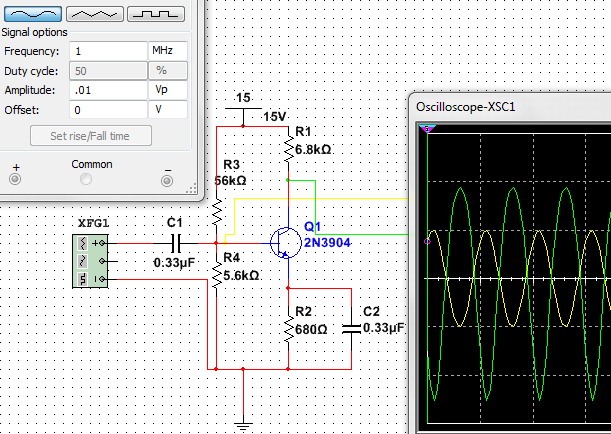
\includegraphics[width=.5\textwidth]{Transistor_2N3904.png}
\caption{\label{fig:Transistor_2N3904}2N3904 Common Emitter Amplifier circuit with theoretical osiciloscope readings showing the clipping problem seen with our circuit - MultiSim Blue v13, Yellow - 20mV/Div, Green - 1V/Div}
\end{figure}

\begin{figure}
\centering
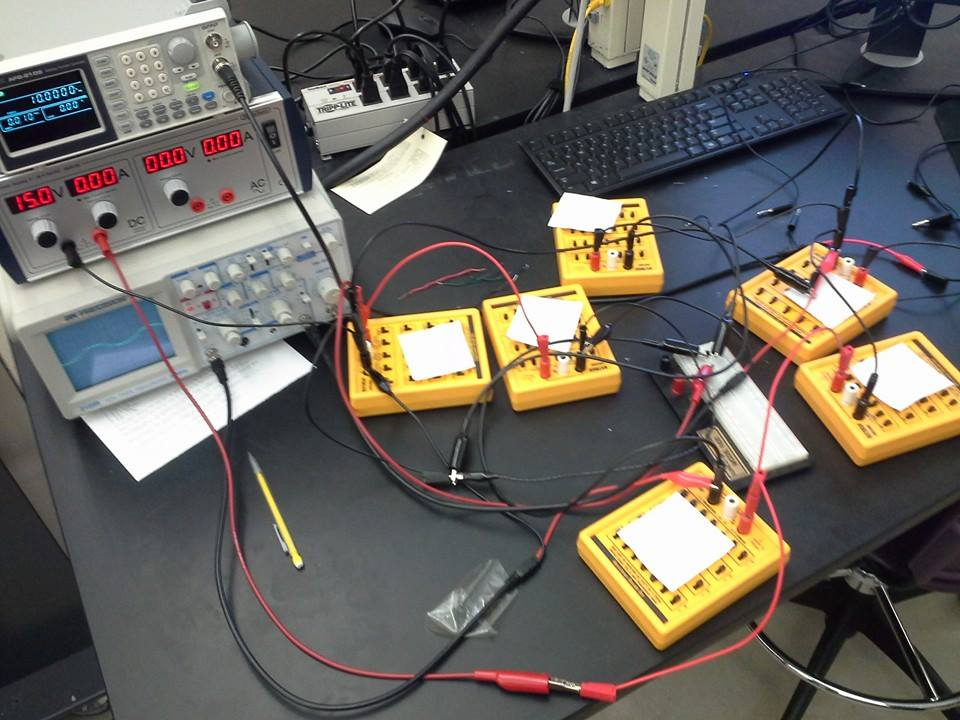
\includegraphics[width=.4\textwidth]{2n3904_-_Setup.jpg}
\caption{\label{fig:2n3904_-_Setup}Picture of actual circuit design}
\end{figure}

\subsection{Circuit Explanation}

This circuit is designed to amplify the input signal, and change the output signal to have \({pi}/2\) phase change relative to the input signal. Thus, inverting the signal.

For our circuit, we saw many different lines, all around where the signal should have been.  It was as if the signal had been stretched out over a certain range of possibilities, creating a kind of shadow or echo on the osciloscope.  See Figure 3.

The optput of the circuit is read from the Green wire in Figure 1.  The Input is read from the Yellow wire.  Comparing signals from Figure 3 and Figure 1, we see how our real circuit performs as expected, but with it's shadow.

\begin{figure}
\centering
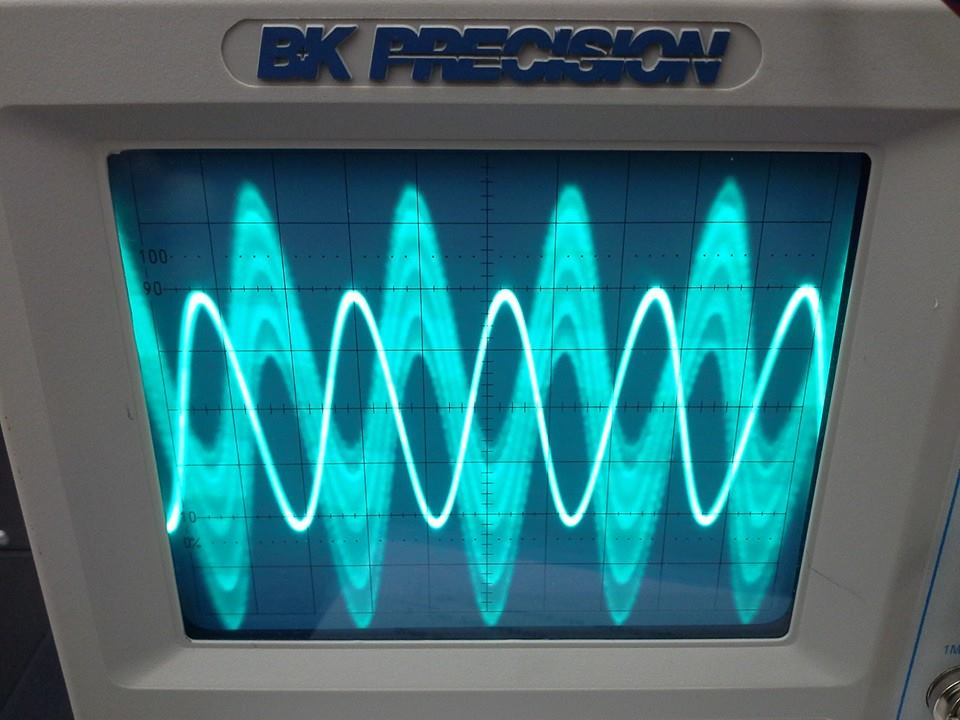
\includegraphics[width=.5\textwidth]{Weird-Signal.jpg}
\caption{\label{fig:Weird-Signal}2N3904 Common Emitter Amplifier circuit causing us a real headache - Photo taken during lab}
\end{figure}

\section{Discussion}

\begin{itemize}
\item 1) How does your circuits behave at low-, mid-, and high-frequencies? (i.e.
does the gain change as you change the frequency?)

The circuit at very low frequencies does not amplify the circuit.  This can be fixed by changing the values of the input and output capacitors.  At mid frequencies (100hz-20khz) the amplification is 10 times the input signal.  At higher frequencies (20khz-3Mhz) the amplification increases to 100 times the input signal.  Above this the signal becomes smaller, however this can be adjusted by changing the value for the output capaictor.  Both of the capacitors are important in controlling the critical frequencies at which the signals will change.

\item 2) Can you measure the input impedance of your amplifier?

We were unable to measure it, however, using online resources I have found the values for the transistor.  Using these values and the known values of the transistor circuit I can solve for the input impedence by,

\[Rin= Hfe*RE\]

Hfe of the 2N3904 resistor according to Korea Electronics Co. can vary based on the current and voltage at the collectors \todo{The current measured is IC, and the voltage VCE}pin.  This value can be between 40 to 300.  Using their datasheet the transistor appears to be running with an Hfe between 40 to 70 (approximately 200uA).  This could mean, 

\[27200(Ohm)<Rin<47600 (Ohm)\]

However, we were unable to measure this to verify the result.

\item 3) Can you measure the output impedance of your amplifier?

For the output impedance I used the value of the collector's resistor.  

\[Zout=6.8k\]

\end{itemize}

\section{Conclusion}

We were able to construct a working amplifier circuit.  However, the circuit did not perform optimally, and only showed a part of what we were hoping to create.  The distortion was likely caused due to too many wires being used in the same node on one part of a circuit.  All of which were going into one another.    

However, we were able to show that the amplification increases between a certain set of frequencies, and were able to control how that amplification functioned for different frequencies.  This could be very important in the designing of large and complicated circuits like Operational Amplifiers and the isolation of very specific signals.

\end{document}

\subsection{How to Make Tables}

Use the table and tabular commands for basic tables --- see Table~\ref{tab:widgets}, for example.

\begin{table}
\centering
\begin{tabular}{l|r}
Item & Quantity \\\hline
Widgets & 42 \\
Gadgets & 13
\end{tabular}
\caption{\label{tab:widgets}An example table.}
\end{table}

\subsection{How to Write Mathematics}

\LaTeX{} is great at typesetting mathematics. Let $X_1, X_2, \ldots, X_n$ be a sequence of independent and identically distributed random variables with $\text{E}[X_i] = \mu$ and $\text{Var}[X_i] = \sigma^2 < \infty$, and let
$$S_n = \frac{X_1 + X_2 + \cdots + X_n}{n}
      = \frac{1}{n}\sum_{i}^{n} X_i$$
denote their mean. Then as $n$ approaches infinity, the random variables $\sqrt{n}(S_n - \mu)$ converge in distribution to a normal $\mathcal{N}(0, \sigma^2)$.

\subsection{How to Make Sections and Subsections}

Use section and subsection commands to organize your document. \LaTeX{} handles all the formatting and numbering automatically. Use ref and label commands for cross-references.

\subsection{How to Make Lists}

You can make lists with automatic numbering \dots

\begin{enumerate}
\item Like this,
\item and like this.
\end{enumerate}
\dots or bullet points \dots
\begin{itemize}
\item Like this,
\item and like this.
\end{itemize}
\dots or with words and descriptions \dots
\begin{description}
\item[Word] Definition
\item[Concept] Explanation
\item[Idea] Text
\end{description}

We hope you find write\LaTeX\ useful, and please let us know if you have any feedback using the help menu above.

\end{document}